\documentclass[tikz,border=8pt]{standalone}
\usetikzlibrary{arrows.meta,calc}
\definecolor{bg}{HTML}{FFFFFF}
\definecolor{sphere}{HTML}{EAF1F8}
\definecolor{sphereedge}{HTML}{4A5A6A}
\definecolor{eq}{HTML}{7A8A9A}
\definecolor{axis}{HTML}{233044}
\definecolor{state}{HTML}{C0392B}
\definecolor{theta}{HTML}{2A6F97}
\definecolor{phi}{HTML}{2E7D4F}
\definecolor{proj}{HTML}{8E44AD}
\begin{document}
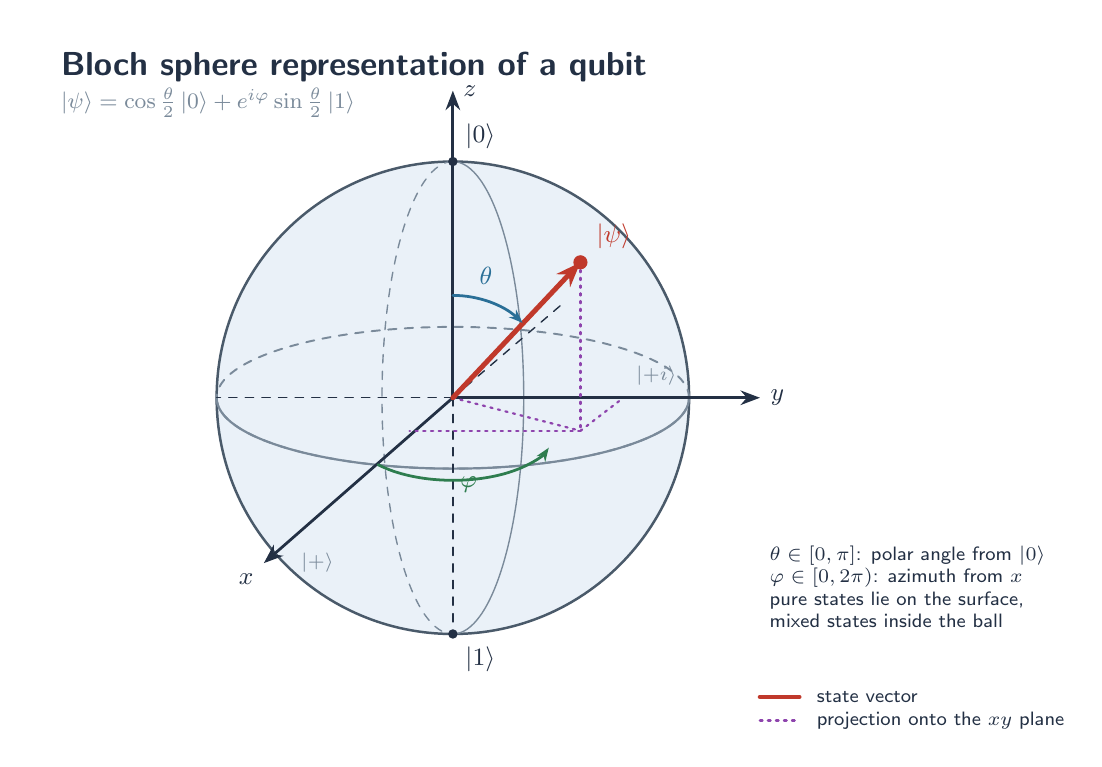
\begin{tikzpicture}[x=1cm,y=1cm,line cap=round,line join=round,
  axisarrow/.style={-{Stealth[length=7pt]},line width=1pt,axis},
  ang/.style={-{Stealth[length=5pt]},line width=1pt}]
  \fill[bg] (-6,-4.5) rectangle (6,4.5);
  \node[font=\sffamily\bfseries\large,text=axis,anchor=west] at (-5.7,4.0) {Bloch sphere representation of a qubit};
  \node[font=\sffamily\footnotesize,text=eq,anchor=west] at (-5.7,3.55) {$|\psi\rangle = \cos\frac{\theta}{2}\,|0\rangle + e^{i\varphi}\sin\frac{\theta}{2}\,|1\rangle$};

  % ---- sphere (radius 3, centred at (-0.6,-0.2)) ----
  \coordinate (O) at (-0.6,-0.2);
  \def\R{3}
  \pgfmathsetmacro{\Rr}{3}
  \fill[sphere] (O) circle (\R);
  \draw[sphereedge,line width=0.9pt] (O) circle (\R);
  % equator ellipse (front solid, back dashed)
  \draw[eq,line width=0.7pt,dashed] ($(O)+(-\R,0)$) arc (180:360:3 and 0.9);
  \draw[eq,line width=0.7pt,dashed] ($(O)+(\R,0)$) arc (0:180:3 and 0.9);
  \draw[eq,line width=0.8pt] ($(O)+(-\R,0)$) arc (180:360:3 and 0.9);
  % meridian (x-z plane) faint
  \draw[eq,line width=0.5pt,dashed] ($(O)+(0,\R)$) arc (90:270:0.9 and 3);
  \draw[eq,line width=0.5pt] ($(O)+(0,-\R)$) arc (-90:90:0.9 and 3);

  % ---- axes ----
  % z (up), y (right), x (toward viewer: down-left)
  \draw[axisarrow] (O) -- ($(O)+(0,\R+0.9)$) node[right,font=\sffamily\small] {$z$};
  \draw[axisarrow] (O) -- ($(O)+(\R+0.9,0)$) node[right,font=\sffamily\small] {$y$};
  \draw[axisarrow] (O) -- ($(O)+(-2.4,-2.1)$) node[below left,font=\sffamily\small] {$x$};
  \draw[axis,dashed,line width=0.5pt] (O) -- ($(O)+(0,-\R)$);
  \draw[axis,dashed,line width=0.5pt] (O) -- ($(O)+(-\R,0)$);
  \draw[axis,dashed,line width=0.5pt] (O) -- ($(O)+(1.4,1.2)$);

  % basis-state labels
  \fill[axis] ($(O)+(0,\R)$) circle (0.06) node[above right=1pt,font=\sffamily\small] {$|0\rangle$};
  \fill[axis] ($(O)+(0,-\R)$) circle (0.06) node[below right=1pt,font=\sffamily\small] {$|1\rangle$};
  \node[font=\sffamily\scriptsize,text=eq] at ($(O)+(-2.05,-1.85)$) [below right] {$|{+}\rangle$};
  \node[font=\sffamily\scriptsize,text=eq] at ($(O)+(\R,0)$) [above left=1pt] {$|{+}i\rangle$};

  % ---- state vector |psi> ----
  % theta = 50 deg from z, phi = 40 deg from x (projected)
  % projected direction of the state: computed in 2D
  \coordinate (P) at ($(O)+(1.62,1.72)$);
  \coordinate (Pxy) at ($(O)+(1.62,-0.42)$);
  % projection helpers (purple dotted)
  \draw[proj,dotted,line width=0.8pt] (P) -- (Pxy);
  \draw[proj,dotted,line width=0.8pt] (O) -- (Pxy);
  \draw[proj,dotted,line width=0.8pt] (Pxy) -- ($(O)+(2.14,-0.02)$);
  \draw[proj,dotted,line width=0.8pt] (Pxy) -- ($(O)+(-0.55,-0.42)$);
  % vector
  \draw[-{Stealth[length=9pt]},line width=1.8pt,state] (O) -- (P);
  \fill[state] (P) circle (0.09);
  \node[font=\sffamily\small,text=state,anchor=south west] at ($(P)+(0.08,0.05)$) {$|\psi\rangle$};

  % ---- angles ----
  % theta: arc from z-axis to the vector (in the plane containing z and P)
  \draw[ang,theta] ($(O)+(0,1.3)$) arc (90:47:1.3);
  \node[font=\sffamily\small,text=theta] at ($(O)+(0.42,1.55)$) {$\theta$};
  % phi: arc in the equatorial plane from x toward the projection
  \draw[ang,phi] ($(O)+(-0.95,-0.85)$) arc (222:342:1.28 and 0.6);
  \node[font=\sffamily\small,text=phi] at ($(O)+(0.2,-1.1)$) {$\varphi$};

  % ---- legend / notes ----
  \node[font=\sffamily\scriptsize,text=axis,anchor=west,align=left] at (3.3,-2.6) {$\theta \in [0,\pi]$: polar angle from $|0\rangle$\\$\varphi \in [0,2\pi)$: azimuth from $x$\\pure states lie on the surface,\\mixed states inside the ball};
  \draw[state,line width=1.6pt] (3.3,-4.0) -- (3.8,-4.0); \node[font=\sffamily\scriptsize,text=axis,anchor=west] at (3.9,-4.0) {state vector};
  \draw[proj,dotted,line width=0.9pt] (3.3,-4.3) -- (3.8,-4.3); \node[font=\sffamily\scriptsize,text=axis,anchor=west] at (3.9,-4.3) {projection onto the $xy$ plane};
\end{tikzpicture}
\end{document}
